\documentclass[11pt]{article}
\usepackage[margin=.8in]{geometry}
\usepackage{amsmath,amssymb,graphicx,hyperref,array}
\DeclareUnicodeCharacter{2082}{\ensuremath{{}_2}}
\setlength{\parindent}{0pt}
\setlength{\parskip}{6pt}
\begin{document}
\begin{center}
{\Large Actual paired support factors out of both coefficients}\\
23 November 2026 --- fixed-support local unsigned Lean evidence
\end{center}
\textbf{Construction.}
Let \(K\) be a field with \(2\ne0\), let \(f\) have degree three,
and retain the actual target and three opposite point-pairs, nonzero ordinates,
distinct target abscissa and original full mixed-jet constraints.
For the actual original-kernel witness, the remainder is \(A+BY\).
Define
\[
 G=\prod_{x\in S}(X-x),\qquad D=G^4,\qquad
 A'=A/_{\!m}D,\quad B'=B/_{\!m}D,\quad N'=A'^2-fB'^2.
\]
Actual monic division constructs these coefficients. Lean derives
\[
 A=DA',\quad B=DB',\quad \deg A'\le3,\quad \deg B'\le1,\quad
 N=D^2N'\ne0,\quad \deg N'\le6,\quad (X-x_t)^4\mid N'.
\]
No successful divisor or quotient is supplied
(PCC-20261123-a66281 and 2aebc0) [pcc:unverified].

\begin{center}
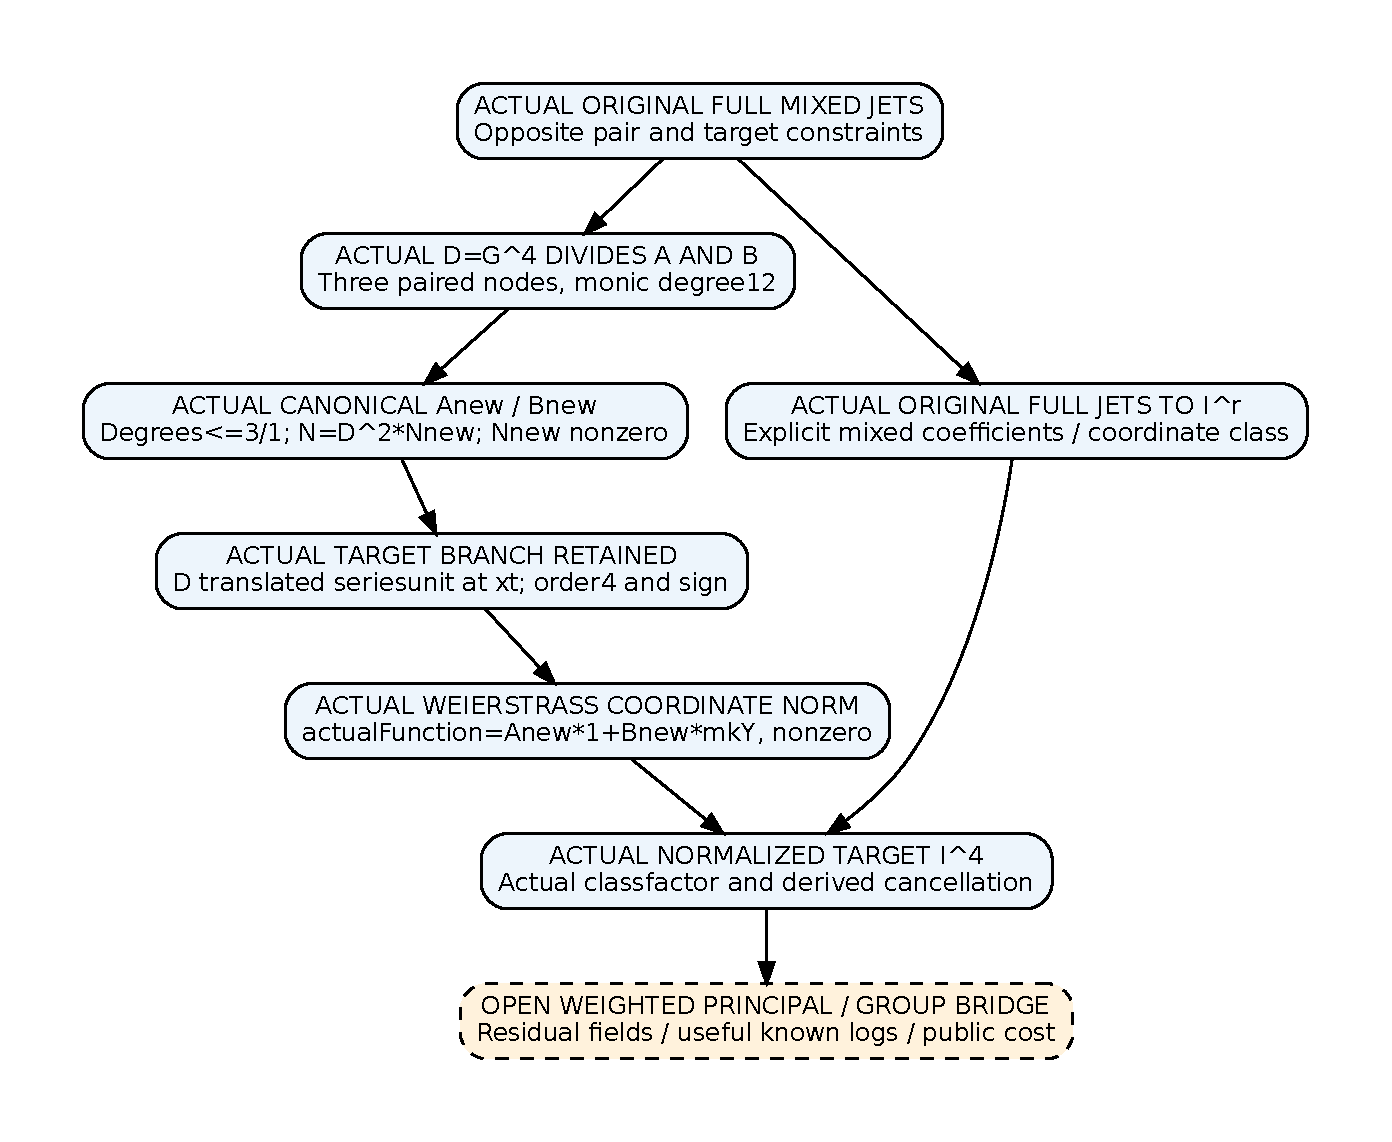
\includegraphics[height=5.1in,width=.95\linewidth,keepaspectratio]{normalization-dependencies-001.pdf}
\end{center}
Solid boxes are accepted actual constructions; dashed boxes retain their stated
open obligations. The diagram describes mathematical implications,
not timings or a runtime improvement [pcc:unverified].

\newpage
\begin{center}{\Large The actual algebra and target sign are retained}\end{center}

\textbf{1. Derive both coefficient factors.}
At an actual paired point, the existing complete-ring theorem constructs
\(s=y+Tu\) with \(s^2=f(x+T)\). Original full multiplicity \(r\) puts both
original branch evaluations in \((T^r)\).
Evaluation at the actual root identifies them with \(A(x+T)\pm
B(x+T)s\). Their difference is \(2sB(x+T)\).
The constant coefficient \(2y\ne0\) makes \(2s\) a unit, so
\(T^r\mid B(x+T)\). Subtraction gives the same order for \(A\).
The previously audited exact translation/root-power equivalence gives
\((X-x)^r\mid A,B\). Distinct abscissas make the factors coprime;
their product for \(r=4\) is the actual monic \(D\) of degree twelve
(PCC-20261123-a66281) [pcc:unverified].

\textbf{2. Construct canonical normalized coefficients.}
Actual monic division reconstructs \(A=DA'\) and \(B=DB'\).
The existing exact degree formula for monic division, with original degree
bounds fifteen and thirteen, gives degrees at most three and one.
Substitution gives the actual identity \(N=D^2N'\);
the existing nonzero actual norm forces \(N'\ne0\), and the coefficient
degree bounds give \(\deg N'\le6\).
Coprimality of \(D\) and \(X-x_t\) retains the target norm factor of
power four (PCC-20261123-2aebc0) [pcc:unverified].

\textbf{3. Preserve the actual target branch.}
Because \(x_t\notin S\), the actual translated series \(D(x_t+T)\) has
nonzero constant coefficient and is a unit.
The exact original evaluation equals that unit times
\(A'(x_t+T)+B'(x_t+T)s_t\), for the actual constructed target branch \(s_t\).
Cancellation retains both its sign and order four; this is stronger than
asserting a root of the norm alone (PCC-20261123-00ed3f) [pcc:unverified].

\textbf{4. Bind an explicit actual Weierstrass function.}
Use the explicit polynomial \(f=X^3+a_2X^2+a_4X+a_6\) of actual \(W\),
with \(a_1=a_3=0\), and construct
\(h=A'\cdot1+B'\cdot\operatorname{mk}(Y)\).
The public Mathlib basis-norm formula gives its actual algebra norm \(N'\);
nonzero \(N'\) makes \(h\ne0\). The actual equation equality, original/remainder
class equality and canonical quotients give
\(\operatorname{mk}(p)=\operatorname{mk}(D)h\).
These are exact coordinate-ring identities, not similarities to a norm formula
(PCC-20261123-524105) [pcc:unverified].

\textbf{5. Direct original ideal powers.}
A new generic owner theorem expands actual polynomial evaluation into
coefficients: if all terms below total degree \(r\) vanish and both arguments
belong to \(I\), the actual evaluation belongs to \(I^r\).
The consumer derives its shifted coefficients from original full jets,
identifies actual coordinate generators and the actual quotient class,
and obtains original class membership in \(I^r\), for all \(r\).
No local-series faithfulness or ideal-power witness is assumed
(PCC-20261123-5ecf4f) [pcc:unverified].

\newpage
\begin{center}{\Large Evidence scope and the next group obligation}\end{center}

\textbf{Proof map.}
The accepted primary source068/build072/local036 contains182 statements,
thirty-five new since147. Its new namespaces are:
\begin{center}
\begin{tabular}{lr}
\texttt{OrientationActualPairedCoefficients}&7\\
\texttt{OrientationActualNormalizedNorm}&7\\
\texttt{OrientationActualNormalizedBranch}&5\\
\texttt{OrientationActualCoordinateNorm}&4\\
\texttt{OrientationActualPointIdealPowers}&2\\
\texttt{OrientationActualExplicitCoordinate}&10
\end{tabular}
\end{center}
The run exits zero; every printed dependency is a standard foundation:
\texttt{propext}, \texttt{Classical.choice} and \texttt{Quot.sound}.
The final run has zero warnings; the earlier181 run retains one style warning.
This is local unsigned data, outside the historical shared Transport53/57
audit/fresh; no independent signed standing follows [pcc:unverified].

Separate owner \texttt{PolynomialBivariateIdealOrder} is committed at
\texttt{64bda75}. Its focused build and unchanged actual audit report one
theorem, zero failing and zero extra trusted. Its single-page report is
inspected. PCC-20261123-f68d78 and 22d015 bind standalone/module evidence.
Lean4.35.0, Mathlib revision \texttt{cfc55fc} and full exact dependency
digests/read-only qualifiers are pinned in the receipts [pcc:unverified].

\textbf{Actual normalized ideal power.}
Original full jets give \(\operatorname{mk}(p)\in I^4\).
The actual class factor above and derived polynomial coprimality of \(D\)
with \((X-x_t)^4\) give a coordinate-ring Bezout identity.
Since the actual \(X-x_t\) class to power four belongs to \(I^4\), ideal
closure and that identity cancel \(\operatorname{mk}(D)\).
Thus the actual nonzero \(h\) has norm degree at most six and belongs to
the actual target point ideal fourth power. No successful ideal-power
witness is supplied (PCC-20261123-524105) [pcc:unverified].

The final endpoint derives the original point equations from actual
\(W.\mathrm{Nonsingular}\) target and paired-point premises and constructs
that nonzero \(h\), retaining all explicit nonzero-ordinate and short-form
conditions (PCC-20261123-f01f40) [pcc:unverified].

\textbf{Group and scalar boundary.}
Existing \texttt{NormGroupBridge} already supplies actual principal-ideal
and group/supplied-label scalar implications.
Its simple-point degree-exhaustion hypotheses are not automatically met by
repeated target multiplicity. A multiplicity-aware actual principal product,
residual degree/field/point analysis and group relation remain to be proved [pcc:unverified].
Residual roots do not supply their discrete logarithms.
Useful known-label base membership, efficient public generation,
coverage/retries and complete expected bit cost remain open.

\textbf{Original criteria.}
General nonsingular \(E/\mathbb F_p\), \(p>3\), prime subgroup order \(r\),
\(\log p=O(\log r)\), public \(P,Q\), no weak-curve or reusable-precomputation
shortcut, and full expected \(\exp(o(\log r))\) bit cost remain unchanged.
A scoped route obstruction would not establish universal nonexistence.
The original nonscalar-origin and rank-directed \(W\)-jet proposals remain
separate unbound mechanisms.

\textbf{Preserved failures and infrastructure.}
Failed057/build060 and061/build065, empty-qualifier admin061,
style-warning058/build062, wrapper failure063/build067 and opaque-alias
failure065/build069 remain exact. Earlier old-alias adapters are retained;
no equality to the new explicit interface is assumed. The missing-namespace
failure067/build071 is preserved as well.
No linter, resource, trust, gate or private-body override was used.
The owner report's failed Unicode/overflow layout remains exact.
A restart was recovered by inspecting the completed original output rather
than repeating its run. Canonical PCC ledger divergence blocks remote
publication only; neither chain is rewritten.
\end{document}
